\documentclass[12pt, a4paper]{report}
\usepackage[T1]{fontenc}
\usepackage[utf8]{inputenc}
\usepackage[margin=2.5cm, top=3cm, bottom=3cm]{geometry}
\usepackage{xcolor}
\usepackage{tikz}
\usetikzlibrary{shapes.geometric, arrows.meta, positioning, calc}
\usepackage{listings}
\usepackage[colorlinks=true, linkcolor=cyancol, urlcolor=cyancol, citecolor=cyancol]{hyperref}
\usepackage{titlesec}
\usepackage{fancyhdr}
\usepackage{amsmath}
\usepackage{amssymb}
\usepackage{booktabs}
\usepackage{tabularx}
\usepackage{array}
\usepackage{colortbl}
\usepackage{enumitem}
\usepackage{float}
\usepackage{setspace}
\usepackage[most]{tcolorbox}

% ─────────────────────────────────────────
% LIGHT THEME - WHITE BACKGROUND, BLACK TEXT
% ─────────────────────────────────────────
\definecolor{darkbg}{HTML}{FFFFFF}
\definecolor{cyancol}{HTML}{0077BB}
\definecolor{softwhite}{HTML}{000000}
\definecolor{dimwhite}{HTML}{333333}
\definecolor{crimsoncolor}{HTML}{CC0000}
\definecolor{embercolor}{HTML}{CC5500}
\definecolor{solarcolor}{HTML}{CC8800}
\definecolor{mosscolor}{HTML}{008800}
\definecolor{cobaltcolor}{HTML}{0055AA}
\definecolor{violetcolor}{HTML}{8800AA}
\definecolor{rosecolor}{HTML}{CC1177}
\definecolor{onyxcolor}{HTML}{555555}
\definecolor{codebg}{HTML}{F5F5F5}
\definecolor{codefg}{HTML}{000000}
\definecolor{codegreen}{HTML}{006600}
\definecolor{codeblue}{HTML}{0055AA}
\definecolor{codeyellow}{HTML}{884400}
\definecolor{codecomment}{HTML}{666666}
\definecolor{sectionline}{HTML}{0077BB}
\definecolor{boxbg}{HTML}{EEEEEE}

\lstdefinelanguage{Dart}{
  morekeywords={abstract,as,assert,async,await,break,case,catch,class,const,
    continue,default,do,dynamic,else,enum,extends,factory,false,final,finally,
    for,Function,get,if,implements,import,in,is,late,library,mixin,new,null,
    on,operator,required,rethrow,return,set,static,super,switch,this,throw,
    true,try,typedef,var,void,while,with,yield,String,int,double,bool,List,
    Map,Set,Future,Stream,Widget,StatelessWidget,StatefulWidget,State,
    BuildContext,Key,override},
  sensitive=true,
  morecomment=[l]{//},
  morecomment=[s]{/*}{*/},
  morestring=[b]",
  morestring=[b]',
}
\lstdefinestyle{dartcode}{
  language=Dart,
  backgroundcolor=\color{codebg},
  basicstyle=\ttfamily\footnotesize\color{codefg},
  keywordstyle=\color{codeblue}\bfseries,
  commentstyle=\color{codecomment}\itshape,
  stringstyle=\color{codegreen},
  numberstyle=\tiny\color{codecomment},
  numbers=left, numbersep=10pt, stepnumber=1,
  frame=none, breaklines=true, tabsize=2,
  showstringspaces=false, keepspaces=true,
  emph={setState,initState,dispose,build,onPressed,onTap},
  emphstyle=\color{codeyellow},
}
\lstdefinestyle{yamlcode}{
  backgroundcolor=\color{codebg},
  basicstyle=\ttfamily\footnotesize\color{codefg},
  commentstyle=\color{codecomment},
  stringstyle=\color{codegreen},
  frame=none, breaklines=true, tabsize=2,
  showstringspaces=false,
}
\lstdefinestyle{bashcode}{
  backgroundcolor=\color{codebg},
  basicstyle=\ttfamily\footnotesize\color{codegreen},
  commentstyle=\color{codecomment},
  frame=none, breaklines=true, tabsize=2,
}

\tcbset{
  cyanbox/.style={
    enhanced, breakable,
    colback=codebg, colframe=cyancol,
    arc=6pt, boxrule=2pt,
    left=8pt, right=8pt, top=6pt, bottom=6pt,
    fonttitle=\bfseries\small\color{cyancol},
    attach boxed title to top left={yshift=-2mm, xshift=6mm},
    boxed title style={colback=codebg, colframe=cyancol, arc=3pt, boxrule=1.5pt},
  },
  theorybox/.style={
    enhanced, breakable,
    colback=boxbg, colframe=violetcolor,
    arc=6pt, boxrule=2pt,
    left=10pt, right=10pt, top=8pt, bottom=8pt,
    fonttitle=\bfseries\color{violetcolor},
    coltext=softwhite,
  },
  notebox/.style={
    enhanced, breakable,
    colback=boxbg, colframe=solarcolor,
    arc=4pt, boxrule=2pt,
    left=8pt, right=8pt, top=6pt, bottom=6pt,
    fonttitle=\bfseries\color{solarcolor},
    coltext=softwhite,
  },
}

\titleformat{\chapter}[display]
  {\normalfont\huge\bfseries\color{softwhite}}
  {\color{cyancol}\Large Chapter \thechapter}{10pt}{\color{softwhite}\Huge}
  [\vspace{2pt}\color{cyancol}\rule{\linewidth}{1.5pt}]
\titleformat{\section}
  {\normalfont\Large\bfseries\color{softwhite}}
  {\color{cyancol}\thesection}{8pt}{}
  [\vspace{1pt}\color{cyancol}\rule{\linewidth}{1pt}]
\titleformat{\subsection}
  {\normalfont\large\bfseries\color{softwhite}}
  {\color{cyancol}\thesubsection}{6pt}{}
\titleformat{\subsubsection}
  {\normalfont\normalsize\bfseries\color{softwhite}}
  {\color{cyancol}\thesubsubsection}{5pt}{}

\pagestyle{fancy}
\fancyhf{}
\renewcommand{\headrulewidth}{0.5pt}
\renewcommand{\headrule}{\color{sectionline}\hrule width\headwidth height\headrulewidth \vspace{-\headrulewidth}}
\fancyhead[L]{\small\color{softwhite}Smart Radio --- Flutter Technical Documentation}
\fancyhead[R]{\small\color{cyancol}\thepage}
\fancyfoot[C]{\color{dimwhite}\small\texttt{ZERO FORMS | ALL SIGNAL | ALWAYS LEARNING}}

\setstretch{1.4}
\setlength{\parskip}{6pt}
\setlength{\parindent}{0pt}
\pagecolor{darkbg}
\color{softwhite}

\newcommand{\pkg}[1]{\texttt{\color{codeblue}#1}}
\newcommand{\file}[1]{\texttt{\color{codegreen}#1}}
\newcommand{\term}[1]{\textit{\color{solarcolor}#1}}
\newcommand{\colordot}[1]{\textcolor{#1}{\rule{8pt}{8pt}}}

\begin{document}

% --- TITLE PAGE
\begin{titlepage}
\centering
\vspace*{1.5cm}
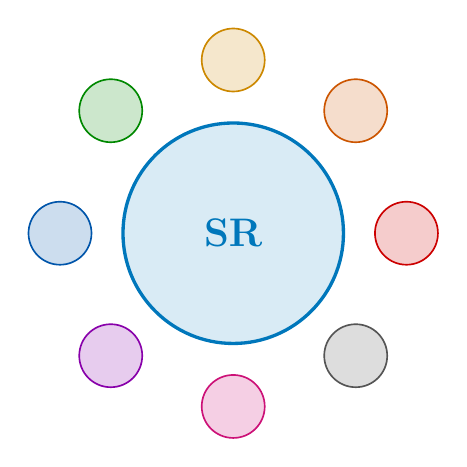
\begin{tikzpicture}
  \node[circle, fill=cyancol!15, draw=cyancol, line width=1.2pt,
        minimum size=2.8cm, font=\Large\bfseries, text=cyancol] (orb) {SR};
  \foreach \angle/\col in {
    0/crimsoncolor, 45/embercolor, 90/solarcolor, 135/mosscolor,
    180/cobaltcolor, 225/violetcolor, 270/rosecolor, 315/onyxcolor} {
    \node[circle, fill=\col!20, draw=\col, line width=0.6pt, minimum size=0.8cm]
      at ([shift={(\angle:2.2cm)}]orb) {};
  }
\end{tikzpicture}

\vspace{1cm}
{\color{cyancol}\small\scshape Flutter Technical Documentation}
\vspace{0.5cm}

{\color{softwhite}\fontsize{32}{38}\selectfont\bfseries Smart Radio}
\vspace{0.3cm}

{\color{softwhite}\large Context-Aware Music Intelligence}\\[4pt]
{\color{softwhite}\large with Personality Color Theory}
\vspace{0.8cm}

{\color{sectionline}\rule{0.6\linewidth}{2pt}}
\vspace{0.5cm}

\begin{tcolorbox}[notebox, width=0.85\linewidth]
\centering\color{softwhite}
A complete guide to building an AI-powered, location-aware,\\
taste-learning music app from scratch in Flutter.\\[4pt]
{\color{softwhite}\small No forms. No surveys. No friction. Only signals.}
\end{tcolorbox}

\vspace{1cm}
{\color{softwhite}\small Version 1.0 \quad|\quad March 2026 \quad|\quad Flutter 3.x / Dart 3.x}
\vfill
{\color{dimwhite}\small\texttt{Built with Claude Sonnet API | Geolocator | SharedPreferences}}
\end{titlepage}

\tableofcontents
\newpage

% =====================================================================
\chapter{The Big Idea}
% =====================================================================

\section{The Problem We Are Solving}

Every music app today does one of two things: it asks you what you want,
or it makes you build a playlist manually. Both create \term{friction}.
The moment a user has to make a deliberate choice, the magic breaks.

\begin{tcolorbox}[theorybox]
\textbf{\color{violetcolor}Core Insight:} The best music curation is invisible.
A great DJ does not ask what you want to hear --- they read the room, watch
energy levels, feel the vibe, and respond. Smart Radio does exactly that,
but through silent data signals collected with zero user effort.
\end{tcolorbox}

\section{The Three-Layer Intelligence Model}

\begin{center}
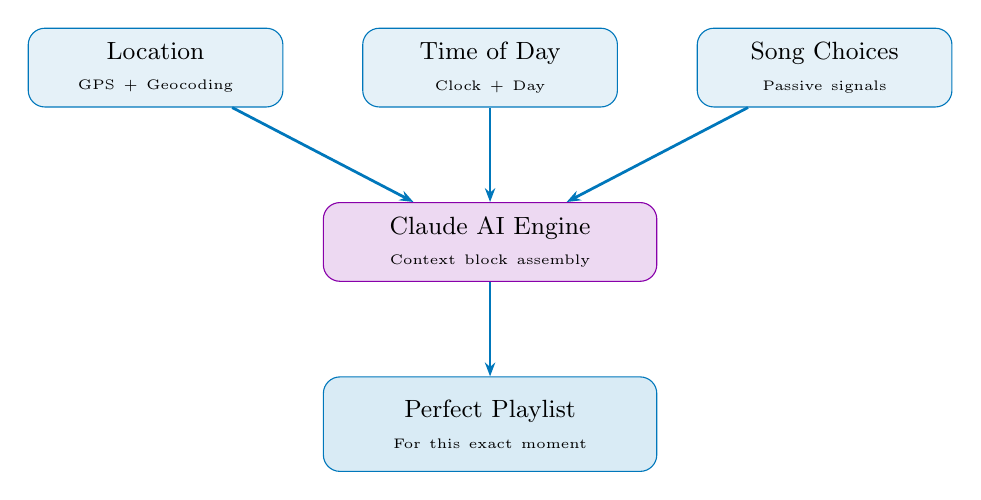
\begin{tikzpicture}[
  box/.style={rectangle, rounded corners=6pt, draw=cyancol, fill=cyancol!10,
              text width=3cm, align=center, minimum height=1cm,
              text=softwhite, font=\small},
  arrow/.style={-{Stealth[length=5pt]}, cyancol, line width=1pt},
]
  \node[box] (L) {Location\\{\tiny GPS + Geocoding}};
  \node[box, right=1cm of L] (T) {Time of Day\\{\tiny Clock + Day}};
  \node[box, right=1cm of T] (C) {Song Choices\\{\tiny Passive signals}};
  \node[box, below=1.2cm of T, fill=violetcolor!15, draw=violetcolor,
        text width=4cm, minimum height=1cm] (ai)
    {Claude AI Engine\\{\tiny Context block assembly}};
  \node[box, below=1.2cm of ai, fill=cyancol!15,
        text width=4cm, minimum height=1.2cm] (out)
    {Perfect Playlist\\{\tiny For this exact moment}};
  \draw[arrow] (L) -- (ai);
  \draw[arrow] (T) -- (ai);
  \draw[arrow] (C) -- (ai);
  \draw[arrow] (ai) -- (out);
\end{tikzpicture}
\end{center}

\subsection{Layer 1 --- Contextual Signals (Immediate)}
Computed on app launch with zero user input:
\begin{itemize}[noitemsep]
  \item \textbf{Location:} GPS coordinates reverse-geocoded to city, region, country
  \item \textbf{Time period:} Hour mapped to an energy label (Morning, Evening, Late Night...)
  \item \textbf{Day type:} Weekday vs.\ weekend changes the social context
\end{itemize}

\subsection{Layer 2 --- Behavioral Learning (Accumulative)}
Every song interaction is a silent data point:
\begin{itemize}[noitemsep]
  \item \textbf{Play} $= +2$ weight on that song's genre/mood/energy axes
  \item \textbf{Like} $= +1$ weight
  \item \textbf{Skip} $= -1$ weight (negative signal, equally valuable)
\end{itemize}

\subsection{Layer 3 --- Personality Color (Emergent)}
Over time, weighted interactions crystallize into a \term{Color DNA}:
an 8-dimensional personality fingerprint that shapes all future recommendations.

% =====================================================================
\chapter{Personality Color Theory}
% =====================================================================

\section{The 8 Color Archetypes}

The Personality Color system maps musical taste to 8 archetypal profiles.
These are not rigid boxes --- every user has a \textbf{blend}. Think of it
as a paint palette: you might be 45\% Cobalt, 30\% Violet, 15\% Onyx.

\begin{table}[H]
\centering
\renewcommand{\arraystretch}{1.5}
\begin{tabularx}{\linewidth}{@{}l l l X@{}}
  \toprule
  \rowcolor{codebg}
  \textbf{\color{cyancol}Color} & \textbf{\color{cyancol}Name} &
  \textbf{\color{cyancol}Tagline} & \textbf{\color{cyancol}Core Genres} \\
  \midrule
  \colordot{crimsoncolor} & Crimson & Raw. Driven. Intense. &
    Hip-Hop, Metal, Trap, Drill \\
  \colordot{embercolor} & Ember & Infectious. Social. Alive. &
    Dance, EDM, Afrobeats, Reggaeton \\
  \colordot{solarcolor} & Solar & Free. Curious. Honest. &
    Indie Pop, Folk, Bedroom Pop \\
  \colordot{mosscolor} & Moss & Grounded. Present. Still. &
    Lo-fi, Ambient Folk, Soft Jazz \\
  \colordot{cobaltcolor} & Cobalt & Deep. Feeling. Real. &
    R\&B, Soul, Neo-soul, Blues \\
  \colordot{violetcolor} & Violet & Strange. Beautiful. Ahead. &
    Experimental, Art Rock, Jazz \\
  \colordot{rosecolor} & Rose & Tender. Warm. Connected. &
    Pop Ballads, K-pop, Love Songs \\
  \colordot{onyxcolor} & Onyx & Nocturnal. Honest. Complex. &
    Post-Punk, Shoegaze, Dark Ambient \\
  \bottomrule
\end{tabularx}
\caption{The 8 Personality Colors and their musical identity}
\end{table}

\section{The Four Scoring Axes}

\begin{center}
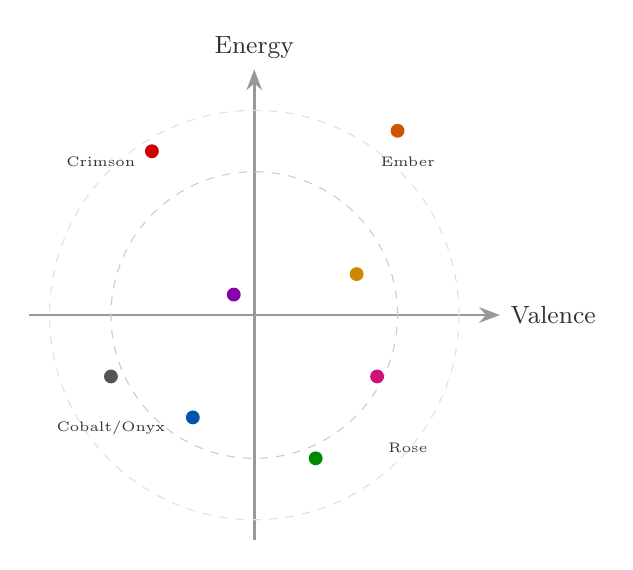
\begin{tikzpicture}[scale=2.6]
  \draw[-{Stealth}, dimwhite!50, line width=1pt]
    (-1.1,0) -- (1.2,0)
    node[right, color=dimwhite, font=\small] {Valence};
  \draw[-{Stealth}, dimwhite!50, line width=1pt]
    (0,-1.1) -- (0,1.2)
    node[above, color=dimwhite, font=\small] {Energy};
  \draw[dimwhite!25, dashed] (0,0) circle (0.7);
  \draw[dimwhite!15, dashed] (0,0) circle (1.0);
  \node[font=\tiny, color=dimwhite] at ( 0.75, 0.75) {Ember};
  \node[font=\tiny, color=dimwhite] at (-0.75, 0.75) {Crimson};
  \node[font=\tiny, color=dimwhite] at ( 0.75,-0.65) {Rose};
  \node[font=\tiny, color=dimwhite] at (-0.7,-0.55) {Cobalt/Onyx};
  \foreach \x/\y/\col in {
    -0.5/0.8/crimsoncolor,  0.7/0.9/embercolor,
     0.5/0.2/solarcolor,    0.3/-0.7/mosscolor,
    -0.3/-0.5/cobaltcolor, -0.1/0.1/violetcolor,
     0.6/-0.3/rosecolor,   -0.7/-0.3/onyxcolor} {
    \node[circle, fill=\col, minimum size=5pt, inner sep=0pt] at (\x,\y) {};
  }
\end{tikzpicture}
\end{center}

\begin{tcolorbox}[cyanbox, title=Color Score Formula]
\begin{align}
  \text{Color Score}_c &= \sum_{i=1}^{N}\, w_i \cdot \mathbf{1}
    \bigl[\text{song}_i \in \text{Color}_c\bigr] \\[6pt]
  \text{Color Weight}_c &= \frac{\max(0,\;\text{Color Score}_c)}
    {\displaystyle\sum_j \max(0,\;\text{Color Score}_j)} \\[6pt]
  \text{Dominant Color} &= \underset{c}{\arg\max}\;\text{Color Weight}_c
\end{align}
{\color{softwhite}Where $w_i \in \{-1, +1, +2, +3\}$ depending on interaction type.}
\end{tcolorbox}

\section{Decision Tree: From Song to Color}

\begin{center}
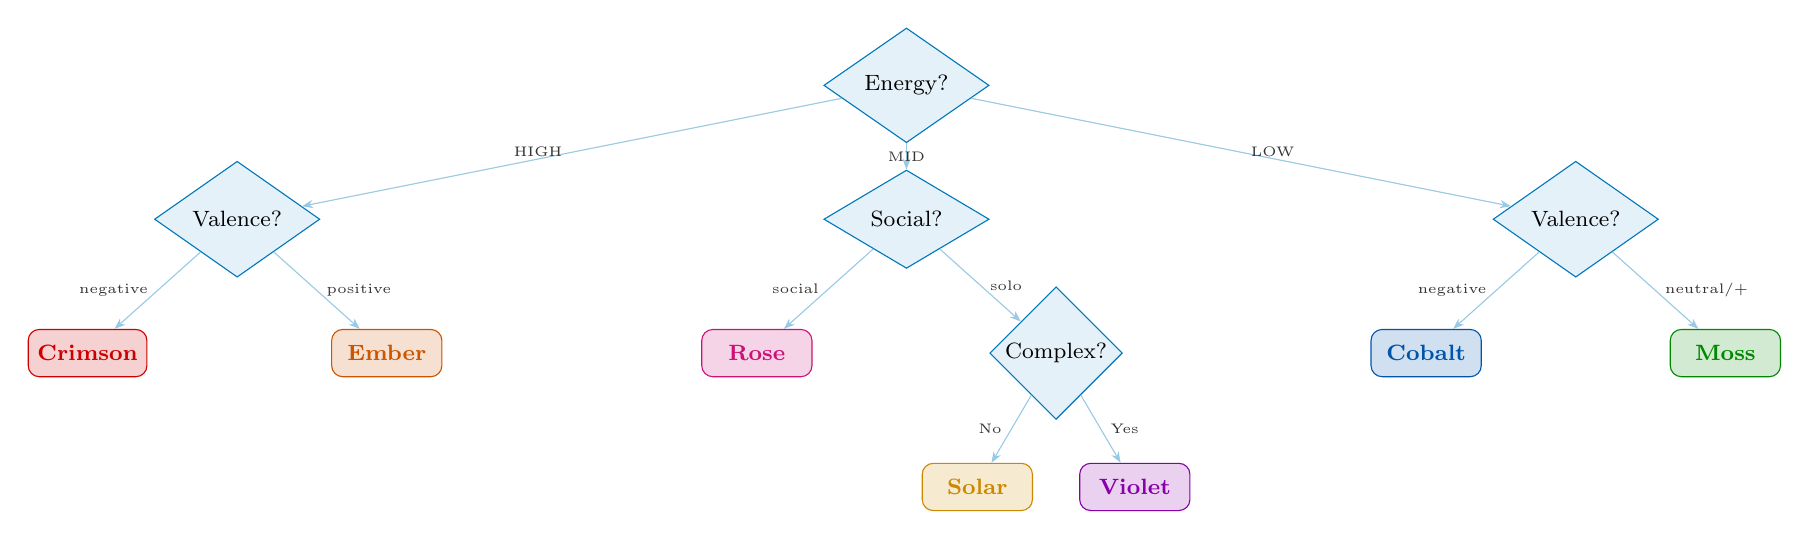
\begin{tikzpicture}[
  level distance=1.7cm,
  level 1/.style={sibling distance=8.5cm},
  level 2/.style={sibling distance=3.8cm},
  level 3/.style={sibling distance=2cm},
  every node/.style={font=\footnotesize},
  dec/.style={diamond, draw=cyancol, fill=cyancol!10, text=softwhite,
              minimum width=2.1cm, minimum height=0.8cm, align=center, inner sep=1pt},
  leaf/.style={rectangle, rounded corners=4pt, draw=#1, fill=#1!18, text=#1,
               minimum width=1.4cm, minimum height=0.6cm, align=center,
               font=\footnotesize\bfseries},
  edge from parent/.style={draw=cyancol!40, -{Stealth[length=4pt]}, thin},
  lbl/.style={font=\tiny, color=dimwhite},
]
  \node[dec] {Energy?}
    child {
      node[dec] {Valence?}
      child { node[leaf=crimsoncolor]{Crimson}
              edge from parent node[left, lbl]{negative} }
      child { node[leaf=embercolor]{Ember}
              edge from parent node[right, lbl]{positive} }
      edge from parent node[left, lbl]{HIGH}
    }
    child {
      node[dec] {Social?}
      child { node[leaf=rosecolor]{Rose}
              edge from parent node[left, lbl]{social} }
      child {
        node[dec, minimum width=1.6cm]{Complex?}
        child { node[leaf=solarcolor]{Solar}
                edge from parent node[left, lbl]{No} }
        child { node[leaf=violetcolor]{Violet}
                edge from parent node[right, lbl]{Yes} }
        edge from parent node[right, lbl]{solo}
      }
      edge from parent node[lbl]{MID}
    }
    child {
      node[dec] {Valence?}
      child { node[leaf=cobaltcolor]{Cobalt}
              edge from parent node[left, lbl]{negative} }
      child { node[leaf=mosscolor]{Moss}
              edge from parent node[right, lbl]{neutral/+} }
      edge from parent node[right, lbl]{LOW}
    };
\end{tikzpicture}
\end{center}

\begin{tcolorbox}[notebox]
\textbf{\color{solarcolor}Note on Onyx:} Onyx emerges from the simultaneous
convergence of low energy, negative valence, and low social score.
It cannot be reached through a single binary branch --- requiring multi-axis
convergence makes Onyx the hardest personality type to misclassify.
\end{tcolorbox}

% =====================================================================
\chapter{Flutter Architecture}
% =====================================================================

\section{Project File Tree}

\begin{tcolorbox}[cyanbox, title=Directory Structure]
\begin{lstlisting}[style=bashcode, numbers=none]
smart_radio/
|-- lib/
|   |-- main.dart
|   |-- models/
|   |   `-- models.dart           Song, SongInteraction, TasteProfile
|   |-- services/
|   |   |-- location_service.dart GPS + Reverse geocoding
|   |   |-- ai_service.dart       Claude API integration
|   |   `-- storage_service.dart  SharedPreferences persistence
|   |-- screens/
|   |   `-- home_screen.dart      Main UI
|   `-- widgets/
|       `-- song_card.dart        Expandable song card
|-- android/app/src/main/
|   `-- AndroidManifest.xml       Location permissions
|-- ios/Runner/
|   `-- Info.plist                iOS permission strings
`-- pubspec.yaml
\end{lstlisting}
\end{tcolorbox}

\section{Layer Diagram}

\begin{center}
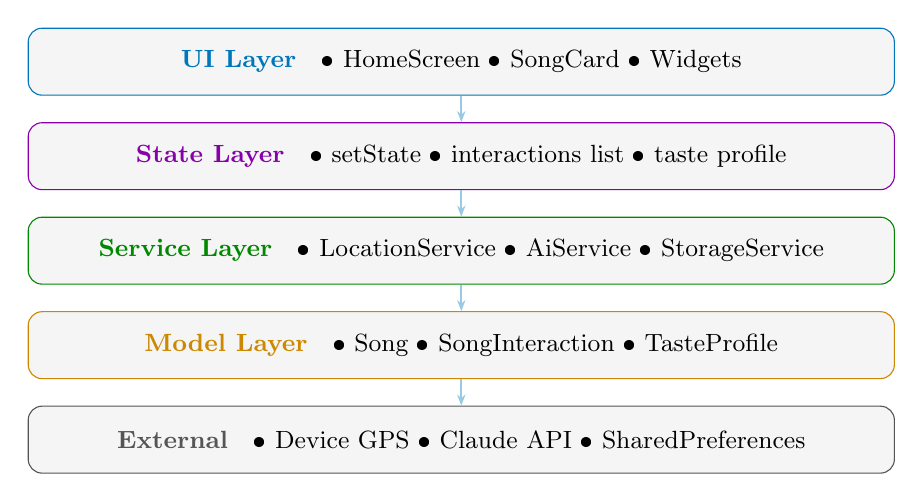
\begin{tikzpicture}[
  layer/.style={rectangle, rounded corners=5pt,
                minimum width=11cm, minimum height=0.85cm,
                align=center, font=\small},
]
  \node[layer, fill=codebg, draw=cyancol] (ui) at (0,0)
    {\color{cyancol}\textbf{UI Layer}\quad
     \color{softwhite}\textbullet{} HomeScreen \textbullet{} SongCard \textbullet{} Widgets};
  \node[layer, fill=codebg, draw=violetcolor] (state) at (0,-1.2)
    {\color{violetcolor}\textbf{State Layer}\quad
     \color{softwhite}\textbullet{} setState \textbullet{} interactions list \textbullet{} taste profile};
  \node[layer, fill=codebg, draw=mosscolor] (service) at (0,-2.4)
    {\color{mosscolor}\textbf{Service Layer}\quad
     \color{softwhite}\textbullet{} LocationService \textbullet{} AiService \textbullet{} StorageService};
  \node[layer, fill=codebg, draw=solarcolor] (model) at (0,-3.6)
    {\color{solarcolor}\textbf{Model Layer}\quad
     \color{softwhite}\textbullet{} Song \textbullet{} SongInteraction \textbullet{} TasteProfile};
  \node[layer, fill=codebg, draw=onyxcolor] (ext) at (0,-4.8)
    {\color{onyxcolor}\textbf{External}\quad
     \color{softwhite}\textbullet{} Device GPS \textbullet{} Claude API \textbullet{} SharedPreferences};
  \foreach \from/\to in {ui/state, state/service, service/model, model/ext} {
    \draw[-{Stealth[length=4pt]}, cyancol!40, line width=0.8pt] (\from) -- (\to);
  }
\end{tikzpicture}
\end{center}

\section{Why Plain setState?}

Smart Radio uses \textbf{local setState} intentionally.
The app has a single screen with a flat, linear data model.
Using BLoC, Riverpod, or Provider would add boilerplate with no practical
benefit at this scale. Rule: reach for \texttt{setState} first,
refactor only when you feel genuine pain.

\begin{tcolorbox}[cyanbox, title=State Variables in HomeScreen]
\begin{lstlisting}[style=dartcode]
class _HomeScreenState extends State<HomeScreen>
    with SingleTickerProviderStateMixin {

  // Layer 1: Contextual signals
  LocationContext? _location;
  late TimeContext _timeCtx;
  bool _locLoading = true;

  // Layer 2: AI output
  PlaylistResult? _playlist;
  bool _loading = false;
  String? _error;

  // Layer 3: Passive taste engine
  List<SongInteraction> _interactions = [];
  final Set<String> _listenedTitles = {};
  int _sessionCount = 0;
}
\end{lstlisting}
\end{tcolorbox}

% =====================================================================
\chapter{Data Models}
% =====================================================================

\section{Song Model}

\begin{tcolorbox}[cyanbox, title=lib/models/models.dart]
\begin{lstlisting}[style=dartcode]
class Song {
  final String title;
  final String artist;
  final String genre;       // "Hip-Hop", "Lo-fi", "EDM"
  final String mood;        // "melancholic", "hype", "chill"
  final String energy;      // "high" | "medium" | "low" | "chill"
  final String emoji;
  final bool trending;
  final String why;         // AI explanation for this pick
  final List<String> signals; // Reasons: time, location, taste

  factory Song.fromJson(Map<String, dynamic> json) => Song(
    title:    json['title']    ?? '',
    artist:   json['artist']   ?? '',
    genre:    json['genre']    ?? '',
    mood:     json['mood']     ?? '',
    energy:   json['energy']   ?? '',
    emoji:    json['emoji']    ?? '*',
    trending: json['trending'] ?? false,
    why:      json['why']      ?? '',
    signals:  List<String>.from(json['signals'] ?? []),
  );

  Map<String, dynamic> toJson() => {
    'title': title, 'artist': artist, 'genre': genre,
    'mood': mood, 'energy': energy, 'emoji': emoji,
    'trending': trending, 'why': why, 'signals': signals,
  };
}
\end{lstlisting}
\end{tcolorbox}

\section{TasteProfile: The Scoring Engine}

\begin{tcolorbox}[cyanbox, title=fromInteractions() --- Passive Learning]
\begin{lstlisting}[style=dartcode]
static TasteProfile fromInteractions(
    List<SongInteraction> interactions) {

  final genres   = <String, int>{};
  final moods    = <String, int>{};
  final energies = <String, int>{};

  for (final i in interactions) {
    if (i.song.genre.isNotEmpty)
      genres[i.song.genre] =
          (genres[i.song.genre] ?? 0) + i.weight;
    if (i.song.mood.isNotEmpty)
      moods[i.song.mood] =
          (moods[i.song.mood] ?? 0) + i.weight;
    if (i.song.energy.isNotEmpty)
      energies[i.song.energy] =
          (energies[i.song.energy] ?? 0) + i.weight;
  }

  // Sort descending, return top 3 per dimension
  List<String> top(Map<String, int> map) =>
      (map.entries.toList()
        ..sort((a, b) => b.value.compareTo(a.value)))
        .take(3)
        .map((e) => e.key)
        .toList();

  return TasteProfile(
    topGenres:   top(genres),
    topMoods:    top(moods),
    topEnergies: top(energies),
  );
}
\end{lstlisting}
\end{tcolorbox}

% =====================================================================
\chapter{Services}
% =====================================================================

\section{LocationService: Why Flutter Works Where Web Failed}

The web prototype failed because browsers sandbox the Geolocation API
and deny it inside embedded iframes. Flutter bypasses this by calling
iOS Core Location and Android LocationManager directly.

\begin{tcolorbox}[cyanbox, title=lib/services/location\_service.dart]
\begin{lstlisting}[style=dartcode]
static Future<LocationContext?> getLocation() async {
  // 1. Check if GPS hardware is enabled
  bool serviceEnabled =
      await Geolocator.isLocationServiceEnabled();
  if (!serviceEnabled) return null;

  // 2. Check / request permission
  LocationPermission permission =
      await Geolocator.checkPermission();
  if (permission == LocationPermission.denied) {
    permission = await Geolocator.requestPermission();
    if (permission == LocationPermission.denied)
      return null;
  }
  if (permission == LocationPermission.deniedForever)
    return null;

  // 3. Get position at medium accuracy (city-level, fast)
  final pos = await Geolocator.getCurrentPosition(
    locationSettings: const LocationSettings(
      accuracy: LocationAccuracy.medium,
      timeLimit: Duration(seconds: 8),
    ),
  );

  // 4. Reverse geocode: (lat, lon) -> "Mumbai, India"
  final placemarks = await placemarkFromCoordinates(
      pos.latitude, pos.longitude);
  final place = placemarks.first;

  return LocationContext(
    city:        place.locality ?? 'Unknown',
    region:      place.administrativeArea ?? '',
    country:     place.country ?? '',
    countryCode: place.isoCountryCode ?? '',
    lat: pos.latitude, lon: pos.longitude,
  );
}
\end{lstlisting}
\end{tcolorbox}

\begin{tcolorbox}[notebox]
\textbf{\color{solarcolor}LocationAccuracy.medium} uses WiFi triangulation
and cell towers --- fast, battery-efficient, and city-level precise.
\texttt{high} activates the GPS chip (5--10 seconds, heavy battery drain).
City-level precision is all we need for regional music curation.
\end{tcolorbox}

\section{AiService: Prompt Architecture}

\begin{tcolorbox}[cyanbox, title=Context Block Assembly]
\begin{lstlisting}[style=dartcode]
final contextLines = <String>[
  'Location: ${location?.fullDisplay ?? "unknown"}',
  'Country code: ${location?.countryCode ?? "unknown"}',
  'Time: ${timeCtx.period} (${DateTime.now().hour}:00), $dayName',
  'Energy: ${timeCtx.energy}, Social: ${timeCtx.social}',
  if (location?.countryCode == 'IN')
    'Include Bollywood and regional Indian music if fitting',
  if (profile.hasData)
    'Taste DNA: genres: ${profile.topGenres.join(", ")}; '
    'moods: ${profile.topMoods.join(", ")}',
  if (interactions.any((i) => i.weight > 0))
    'Played: ${interactions
      .where((i) => i.weight > 0)
      .map((i) => i.song.title).join(", ")}',
  if (interactions.any((i) => i.weight < 0))
    'Skipped: ${interactions
      .where((i) => i.weight < 0)
      .map((i) => i.song.title).join(", ")}',
];
\end{lstlisting}
\end{tcolorbox}

\subsection{The System Prompt}

\begin{tcolorbox}[theorybox]
\textit{``You are a hyper-local, time-aware music curator AI. Pick songs based
on: (1) location --- local and regional hits, what is trending in that area;
(2) time of day --- energy levels and social context; (3) learned user taste
from passive song interactions. Return ONLY valid JSON, no markdown.
Generate exactly 8 songs. Mix: 3 trending in their region,
3 matching taste, 2 wildcard discoveries. Real songs only.''}
\end{tcolorbox}

\section{StorageService: Persistent Taste Memory}

\begin{tcolorbox}[cyanbox, title=lib/services/storage\_service.dart]
\begin{lstlisting}[style=dartcode]
static Future<void> saveInteractions(
    List<SongInteraction> interactions) async {
  final prefs = await SharedPreferences.getInstance();

  // Cap at 100 interactions (FIFO trim)
  // Keeps storage small while preserving recent signals
  final trimmed = interactions.length > 100
      ? interactions.sublist(interactions.length - 100)
      : interactions;

  await prefs.setString(
    'song_interactions',
    jsonEncode(trimmed.map((i) => i.toJson()).toList()),
  );
}
\end{lstlisting}
\end{tcolorbox}

% =====================================================================
\chapter{UI Implementation}
% =====================================================================

\section{Design Principles}

\begin{enumerate}[noitemsep]
  \item Dark ambient background (\texttt{\#0A0F1A}) with \texttt{CustomPainter} glows
  \item Zero-friction first load: auto-geolocate, auto-generate, no onboarding
  \item Progressive disclosure: song cards expand on tap only
  \item Signal bar: persistent strip showing why this playlist was generated
  \item Fonts: Syne (headings) + Instrument Serif (body/reasoning text)
\end{enumerate}

\section{Animated Waveform}

\begin{tcolorbox}[cyanbox, title=Phase-offset waveform bars]
\begin{lstlisting}[style=dartcode]
Row(
  children: List.generate(4, (i) =>
    AnimatedBuilder(
      animation: _waveController,
      builder: (_, __) {
        // Phase offset prevents sync movement
        final val =
            (_waveController.value + i * 0.25) % 1.0;
        final h = 4.0 + 10.0 *
            (val < 0.5 ? val * 2 : (1 - val) * 2);
        return Container(
          width: 3, height: h,
          margin: EdgeInsets.symmetric(horizontal: 1),
          decoration: BoxDecoration(
            color: accent,
            borderRadius: BorderRadius.circular(2),
          ),
        );
      },
    )
  ),
)
\end{lstlisting}
\end{tcolorbox}

\section{Background Glow Painter}

\begin{tcolorbox}[cyanbox, title=CustomPainter with MaskFilter blur]
\begin{lstlisting}[style=dartcode]
@override
void paint(Canvas canvas, Size size) {
  // Primary glow: top-center
  canvas.drawCircle(
    Offset(size.width * 0.5, 0), 200,
    Paint()
      ..color = accent.withOpacity(0.07)
      ..maskFilter =
          const MaskFilter.blur(BlurStyle.normal, 120),
  );
  // Secondary glow: bottom-right
  canvas.drawCircle(
    Offset(size.width * 0.85, size.height * 0.8), 180,
    Paint()
      ..color = const Color(0xFF0EA5E9).withOpacity(0.05)
      ..maskFilter =
          const MaskFilter.blur(BlurStyle.normal, 150),
  );
}
\end{lstlisting}
\end{tcolorbox}

% =====================================================================
\chapter{Platform Permissions}
% =====================================================================

\section{Android}

\begin{tcolorbox}[cyanbox, title=AndroidManifest.xml]
\begin{lstlisting}[style=yamlcode, numbers=none]
<manifest
  xmlns:android="http://schemas.android.com/apk/res/android">

  <uses-permission
    android:name="android.permission.ACCESS_FINE_LOCATION"/>
  <uses-permission
    android:name="android.permission.ACCESS_COARSE_LOCATION"/>
  <uses-permission
    android:name="android.permission.INTERNET"/>

  <application ...>
    <!-- Required for url_launcher on Android 11+ -->
    <queries>
      <intent>
        <action android:name="android.intent.action.VIEW"/>
        <data android:scheme="https"/>
      </intent>
    </queries>
  </application>
</manifest>
\end{lstlisting}
\end{tcolorbox}

\section{iOS}

\begin{tcolorbox}[cyanbox, title=Info.plist (add before closing dict)]
\begin{lstlisting}[style=yamlcode, numbers=none]
<key>NSLocationWhenInUseUsageDescription</key>
<string>
  Smart Radio uses your location to surface locally
  trending songs and region-specific music.
</string>
<key>NSLocationAlwaysAndWhenInUseUsageDescription</key>
<string>
  Smart Radio uses location to keep your music relevant.
</string>
\end{lstlisting}
\end{tcolorbox}

\begin{tcolorbox}[notebox]
\textbf{\color{solarcolor}iOS Gotcha:} Omitting these strings causes a silent
crash on the first \texttt{requestPermission()} call. Apple requires descriptive
text --- vague strings like ``for features'' may be rejected in App Store review.
\end{tcolorbox}

% =====================================================================
\chapter{Dependencies and Setup}
% =====================================================================

\section{pubspec.yaml}

\begin{tcolorbox}[cyanbox, title=pubspec.yaml]
\begin{lstlisting}[style=yamlcode, numbers=none]
name: smart_radio
description: Context-aware music curation. Zero forms.
version: 1.0.0+1
environment:
  sdk: '>=3.0.0 <4.0.0'

dependencies:
  flutter:
    sdk: flutter
  geolocator: ^11.0.0         # Native GPS access
  geocoding: ^3.0.0           # Coordinates -> city name
  http: ^1.2.0                # Claude API HTTP calls
  shared_preferences: ^2.2.3  # Persist taste profile
  google_fonts: ^6.2.1        # Syne + Instrument Serif
  url_launcher: ^6.2.5        # Open YouTube in browser
\end{lstlisting}
\end{tcolorbox}

\section{Package Rationale}

\begin{table}[H]
\centering
\renewcommand{\arraystretch}{1.5}
\begin{tabularx}{\linewidth}{@{}l X@{}}
  \toprule
  \rowcolor{codebg}
  \textbf{\color{cyancol}Package} & \textbf{\color{cyancol}Why this one} \\
  \midrule
  \pkg{geolocator \^{}11} &
    Cross-platform GPS wrapper. Handles full permission flow on iOS and
    Android from a single Dart API. Supports accuracy control. \\
  \pkg{geocoding \^{}3} &
    Converts (lat, lon) to place names using the device's native geocoder.
    No API key needed, works offline. \\
  \pkg{http \^{}1.2} &
    Minimal HTTP client. Sufficient for a single API endpoint.
    Dio would be overkill. \\
  \pkg{shared\_preferences \^{}2.2} &
    Key-value backed by NSUserDefaults (iOS) and SharedPreferences (Android).
    Persists taste DNA across sessions. \\
  \pkg{google\_fonts \^{}6.2} &
    Runtime font loading from CDN. No need to bundle font files in the APK. \\
  \pkg{url\_launcher \^{}6.2} &
    Opens YouTube in external browser. Requires the queries block in
    AndroidManifest for Android 11+. \\
  \bottomrule
\end{tabularx}
\caption{Dependency rationale}
\end{table}

\section{Step-by-Step Setup}

\begin{tcolorbox}[cyanbox, title=Step 1 --- Create and Install]
\begin{lstlisting}[style=bashcode, numbers=none]
flutter create smart_radio
cd smart_radio
flutter pub add url_launcher
flutter pub get
flutter doctor  # check for issues
\end{lstlisting}
\end{tcolorbox}

\begin{tcolorbox}[cyanbox, title=Step 2 --- Add API Key]
\begin{lstlisting}[style=dartcode]
// lib/services/ai_service.dart
static const String _apiKey = 'YOUR_ANTHROPIC_API_KEY';

// Production pattern using dart-define:
// static const String _apiKey =
//     String.fromEnvironment('ANTHROPIC_KEY');
\end{lstlisting}
\end{tcolorbox}

\begin{tcolorbox}[cyanbox, title=Step 3 --- Run and Build]
\begin{lstlisting}[style=bashcode, numbers=none]
flutter run                           # debug
flutter build apk --release          # Android
flutter build ipa                    # iOS (macOS only)

# Inject API key securely at build time
flutter run --dart-define=ANTHROPIC_KEY=sk-ant-...
\end{lstlisting}
\end{tcolorbox}

% =====================================================================
\chapter{Theory and Resources}
% =====================================================================

\section{Music Information Retrieval Background}

\subsection{The Valence--Energy Model}
Spotify's Audio Features API provides two core psychoacoustic dimensions:
\begin{itemize}[noitemsep]
  \item \textbf{Energy} $\in [0,1]$: Perceptual intensity. Fast, loud,
        noisy $\Rightarrow$ high. Quiet, delicate $\Rightarrow$ low.
  \item \textbf{Valence} $\in [0,1]$: Musical positiveness. Happy/cheerful
        $\Rightarrow$ high. Sad/angry/tense $\Rightarrow$ low.
\end{itemize}

Smart Radio approximates these from genre and mood labels returned by Claude,
bypassing the Spotify Audio Analysis OAuth flow. The approximation
is effective for personality clustering.

\subsection{Collaborative vs.\ Content-Based Filtering}

\begin{tcolorbox}[theorybox]
\textbf{\color{violetcolor}Collaborative filtering} recommends based on what
\textit{similar users} liked. Requires large datasets (cold start problem).\\[4pt]
\textbf{\color{violetcolor}Content-based filtering} recommends based on
features of items the user already liked.\\[4pt]
\textbf{\color{violetcolor}Smart Radio hybrid:} content-based scoring
(genre/mood/energy from interactions) enriched by an LLM that implicitly
encodes collaborative knowledge from its training data.
\end{tcolorbox}

\section{Anthropic API Quick Reference}

\begin{tcolorbox}[cyanbox, title=Minimal Dart API Call]
\begin{lstlisting}[style=dartcode]
final response = await http.post(
  Uri.parse('https://api.anthropic.com/v1/messages'),
  headers: {
    'Content-Type':      'application/json',
    'x-api-key':         _apiKey,
    'anthropic-version': '2023-06-01', // Required
  },
  body: jsonEncode({
    'model':      'claude-sonnet-4-20250514',
    'max_tokens': 1000,
    'system':     systemPrompt,
    'messages': [
      {'role': 'user', 'content': contextBlock},
    ],
  }),
);

final data  = jsonDecode(response.body);
final text  = (data['content'] as List)
    .where((c) => c['type'] == 'text')
    .map((c) => c['text'] as String)
    .join('');

// Strip markdown fences, parse JSON
final clean  = text.replaceAll(
    RegExp(r'```json|```'), '').trim();
final parsed = jsonDecode(clean);
\end{lstlisting}
\end{tcolorbox}

\section{Key Resources}

\begin{itemize}[noitemsep]
  \item \href{https://pub.dev/packages/geolocator}{\texttt{pub.dev/packages/geolocator}}
        --- Permission flow and platform setup
  \item \href{https://pub.dev/packages/geocoding}{\texttt{pub.dev/packages/geocoding}}
        --- Reverse geocoding docs
  \item \href{https://docs.flutter.dev/cookbook/networking/fetch-data}
        {flutter.dev: Fetch data from the internet}
  \item \href{https://docs.anthropic.com/en/api/messages}
        {docs.anthropic.com: Messages API reference}
  \item \href{https://docs.flutter.dev/ui/animations}
        {flutter.dev: Animations overview}
  \item \href{https://pub.dev/packages/shared_preferences}
        {\texttt{pub.dev/packages/shared\_preferences}}
\end{itemize}

\section{Feature Roadmap}

\begin{table}[H]
\centering
\renewcommand{\arraystretch}{1.5}
\begin{tabularx}{\linewidth}{@{}l l X@{}}
  \toprule
  \rowcolor{codebg}
  \textbf{\color{cyancol}Feature} & \textbf{\color{cyancol}Priority} &
  \textbf{\color{cyancol}Implementation Path} \\
  \midrule
  Spotify Embed & High &
    \pkg{spotify\_sdk} + OAuth. Replace YouTube with embedded 30s previews. \\
  Offline Color Map & Medium &
    Client-side scoring. No API call for personality screen. \\
  Demographic Hint & Medium &
    Single swipe-to-age-range gesture. One motion, not a form. \\
  Color History Chart & Low &
    Plot Color DNA over time using \pkg{fl\_chart}. \\
  Social Rooms & Future &
    Aggregate anonymized Color profiles by city for hyper-local trending. \\
  \bottomrule
\end{tabularx}
\caption{Feature Roadmap}
\end{table}

% --- FINAL PAGE
\newpage
\thispagestyle{empty}
\begin{center}
\vspace*{4cm}
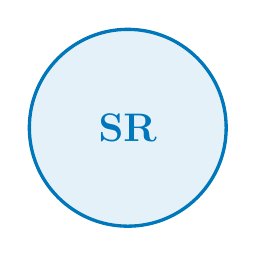
\begin{tikzpicture}
  \node[circle, fill=cyancol!10, draw=cyancol, line width=1.2pt,
        minimum size=2.5cm, font=\Large\bfseries, text=cyancol] {SR};
\end{tikzpicture}

\vspace{1.5cm}
{\color{softwhite}\large\itshape
``Music is the shorthand of emotion.''}\\[4pt]
{\color{dimwhite}\small --- Leo Tolstoy}

\vspace{2cm}
{\color{sectionline}\rule{0.4\linewidth}{2pt}}
\vspace{1cm}

{\color{softwhite}\small\texttt{ZERO FORMS | ALL SIGNAL | ALWAYS LEARNING}}\\[6pt]
{\color{dimwhite}\footnotesize Smart Radio --- Flutter Technical Documentation --- 2026}
\end{center}

\end{document}
